% !TeX root = ../../main.tex
\section{Mechanical drawings}
\label{app:reactor-drawings}

The detailed mechanical design drawings are provided in this section.

\subsection{3D mechanical design and engineering drawings}
\label{app:engineeringdesign}
All dimensions are in the units of mm.
\begin{figure}[h]
    \begin{minipage}[t]{0.6\linewidth}
        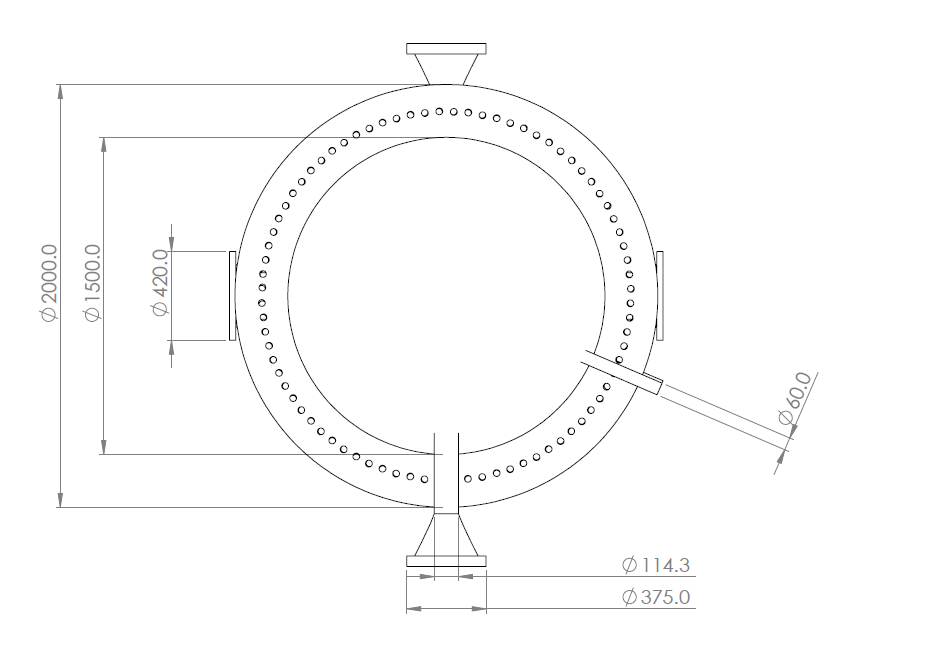
\includegraphics[width=\linewidth]{chapters/2-reaction/figures/FYD reactor bottom view with calc.PNG}
        \caption{Bottom view of the reactor}
        \label{fig:reactorbottom}
    \end{minipage}\hfill
    \begin{minipage}[t]{0.4\linewidth}
        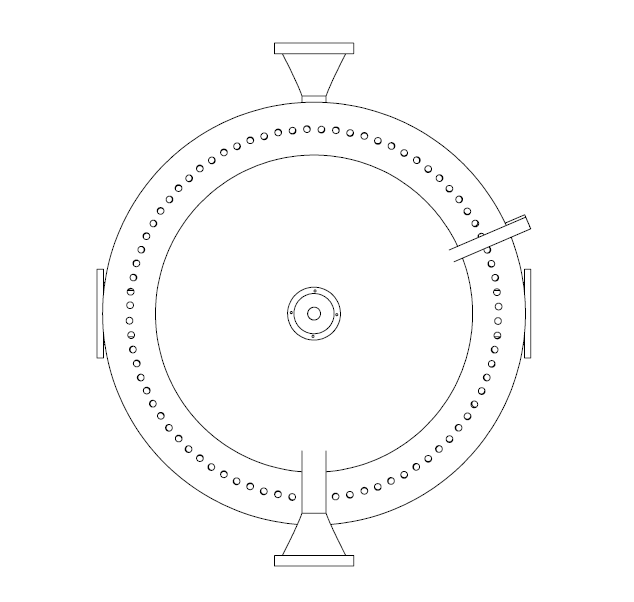
\includegraphics[width=\linewidth]{chapters/2-reaction/figures/FYD reactor top view.PNG}
        \caption{Top view of the reactor}
        \label{fig:reactortop}
    \end{minipage}
\end{figure}
\begin{figure}
    \centering

\end{figure}

\begin{figure}[h]
    \begin{minipage}[t]{0.49\linewidth}
        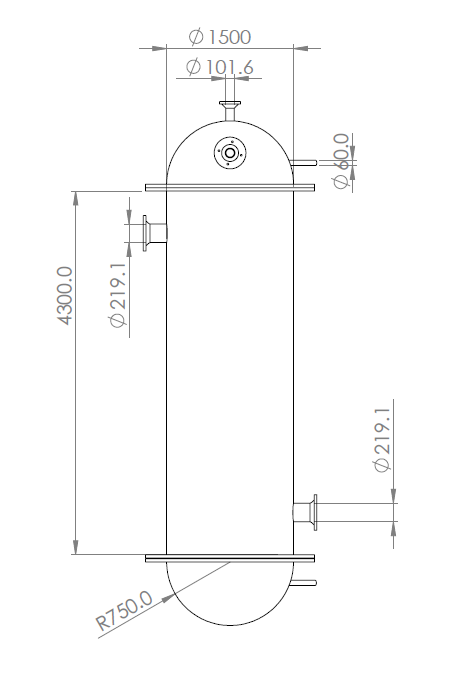
\includegraphics[width=\linewidth]{chapters/2-reaction/figures/FYD reactor right view with calc.PNG}
        \caption{Right view of the reactor}
        \label{fig:reactorright}
    \end{minipage}\hfill
    \begin{minipage}[t]{0.49\linewidth}
        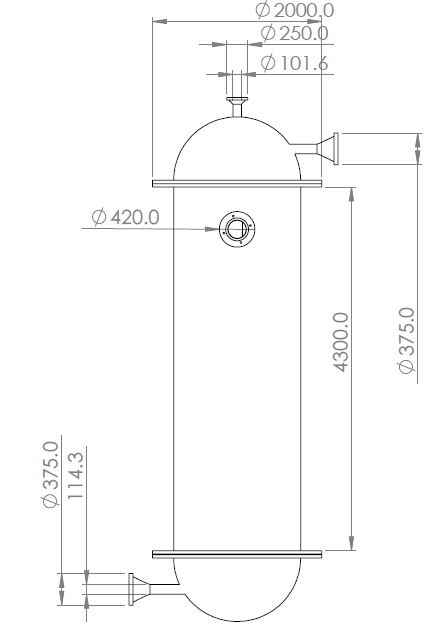
\includegraphics[width=\linewidth]{chapters/2-reaction/figures/FYD reactor left view with calc.PNG}
        \caption{Left view of the reactor}
        \label{fig:reactorleft}
    \end{minipage}
\end{figure}

\begin{figure}
    \centering
    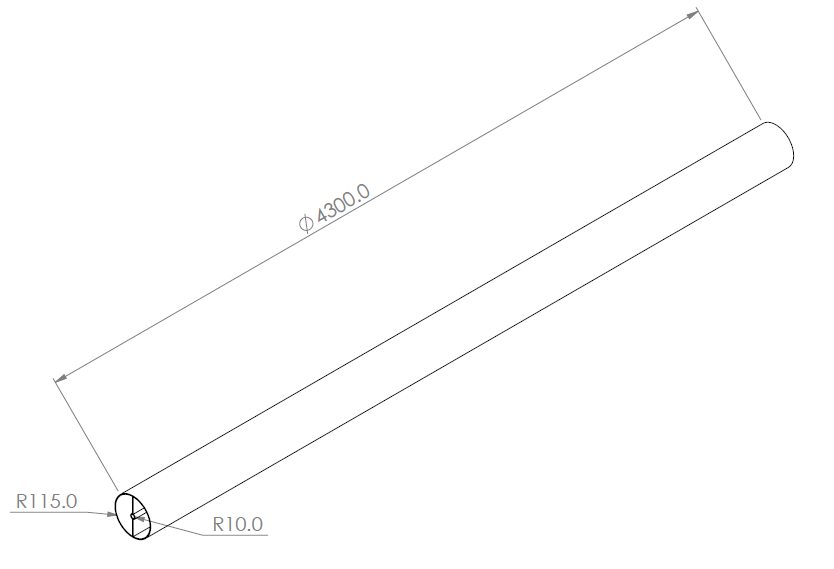
\includegraphics{chapters/2-reaction/figures/FYD solo tube with calc.PNG}
    \caption{Individual reactor tube dimension}
    \label{fig:soloreactor }
\end{figure}